% =========================================================================
% CHAPTER 7
% =========================================================================

\chapter{Evaluierung}
\label{K7}

Dieses Kapitel evaluiert den \textit{pool} und \textit{parallel} Workflow mit mehreren \jobScript s.
Der Webclient wird verwendet um einzelne Test Jobs auszuführen, das CLI um Test Jobs 25 mal auszuführen.
Gemessen wurden neben der Gesamtlaufzeit (\RootJob{} Laufzeit) auch die Laufzeiten der WorkerJobs.
Joblaufzeiten werden immer auf dem Rechner auf dem der Job erstellt wurden gemessen, für \remoteJob s bedeutet das inklusive des Netzwerk Roundtrips.
Das System wird mit beiden Clients einem Stresstest unterzogen, indem WorkerJobs mit minimaler Laufzeit (sie terminieren sobald das onCall Event aufgerufen wird) eingesetzt werden (\ref{M3}, \ref{overload}).
Dieser Stresstest wird mit dem Pool Workflow durchgeführt, da er mehr Netzwerk Messages benötigt.

Ziel der CLI Messungen ist es zu zeigen, dass das \jobScript{} skaliert (\ref{M1}, \ref{M2}).
Jeder Test führt einen Job auf 1, 2 und 4 Worker Devices aus. Auf jedem Worker Device laufen 4 Worker Nodes.
Verteilte Systeme sind nicht zeitlich deterministisch, desshalb werden alle Messungen 25 mal wiederholt.
Die Skalierbarkeit wird mit einem Boxplot der Gesamtlaufzeit mit linearen Achsen, und einem mit logaritmischen Achsen veranschaulicht.
%histogramme der WrokerJobs zeigen unmgebungs eigenschaften, beschreiben vorgangn, lassen auf fehler schließen

Webclient Tests führen ihren Test Job nur ein mal aus.
Der Webclient ist in der lage Gantcharts aus \JobTree s zu generieren.
Diese werden genutzt um die Probleme aufzuzeigen die beim implementieren von \jobScript s entstehen können (\ref{schedulerNeeded}, \ref{overload}).

%ein Script, das einen Bereich der natürlichen Zahlen nach Primzahlen durchsucht (siehe Experiment \ref{M1}),
%und ein weiteres, das einen \rgAlgorithmus{} auf mehrere Input-Dateien anwendet (siehe Experiment \ref{M2}, \ref{M3}).

\begin{table}[H]
\centering

\begin{tabular}{|l|l|l|l|r|r|r|}
\hline
\multicolumn{7}{|l|}{}                                                                                                                                           \\
\multicolumn{7}{|c|}{Webclient Tests}                                                                                                                            \\
\multicolumn{7}{|l|}{}                                                                                                                                           \\ \hline
Abschnitt                             & Wiederh.            & Workflow                  & WorkerJobs          & Worker Nodes & Worker Devices & mean(T) {[}ms{]} \\ \hline
\multirow{3}{*}{\ref{M1} \thumbsup}   & \multirow{9}{*}{25} & \multirow{3}{*}{Parallel} & 4                   & 4        & 1          & 7 004                    \\ \cline{4-7}
                                      &                     &                           & 8                   & 8        & 2          & 3 706                    \\ \cline{4-7}
                                      &                     &                           & 16                  & 16       & 4          & 2 342                    \\ \cline{1-1} \cline{3-7}
\multirow{3}{*}{\ref{M2} \thumbsup}   &                     & \multirow{3}{*}{Pool}     & \multirow{3}{*}{65} & 4        & 1          & 672 136                  \\ \cline{5-7}
                                      &                     &                           &                     & 8        & 2          & 332 253                  \\ \cline{5-7}
                                      &                     &                           &                     & 16       & 4          & 154 961                  \\ \cline{1-1} \cline{3-7}
\multirow{3}{*}{\ref{M3}}             &                     & \multirow{3}{*}{Pool}     & \multirow{3}{*}{20} & 4        & 1          & 103                      \\ \cline{5-7}
                                      &                     &                           &                     & 8        & 2          & 120                      \\ \cline{5-7}
                                      &                     &                           &                     & 16       & 4          & 118                      \\ \hline
\multicolumn{7}{|l|}{}                                                                                                                                           \\
\multicolumn{7}{|c|}{CLI Tests}                                                                                                                                  \\
\multicolumn{7}{|l|}{}                                                                                                                                           \\ \hline
Abschnitt                             & Wiederh.            & Workflow                  & WorkerJobs          & Worker Nodes & Worker Devices & T {[}ms{]}       \\ \hline
\ref{schedulerNeeded}                 & \multirow{2}{*}{1}  & Pool                      & 12                  & 3        & 1          & 21 209                   \\ \cline{1-1} \cline{3-7}
\ref{overload}                        &                     & Pool                      & 20                  & 3        & 1          & 1 064                    \\ \hline
\end{tabular}

\caption{Test Übersicht. Grüner Daumen markiert lineare Skalierbarkeit.}
\label{testtable}
\end{table}


\noindent Als Hardware standen fünf Rechner mit gleicher Ausstattung, jeweils 4 Cores und 16GB RAM, zur Verfügung.
Pro Rechner wurden maximal vier Worker verwendet um Swapping zu vermeiden, denn die \jobScript s verwenden nur einen primitiven \scheduler{}.
Als Betriebssystem wurde Debian Linux verwendet.
Experiment \ref{M2} startet WorkerJobs die auf ein verteiltes Dateisystem (AFS) zugreifen. AFS cached die Lesevorgänge.

%Für die folgenden Experimente wird jeweils ein Histogram der WorkerJob Laufzeiten und ein Boxplot der Gesamtlaufzeit für ein, zwei und vier Rechner gezeigt.
%Weiters wird die Gesamtlaufzeit über der Rechneranzahl auch mit logarithmischen Achsen gezeigt, da in dieser Darstellungsform eine lineare Funktion die lineare Skalierbarkeit besser sichtbar macht.


















\clearpage
\section{CLI Tests}

\subsection{Primzahlen Suche - Parallel Workflow}
\label{M1}

\begin{wrapfigure}{r}{0.45\textwidth}
  \vspace{-30pt}
  \begin{center}
    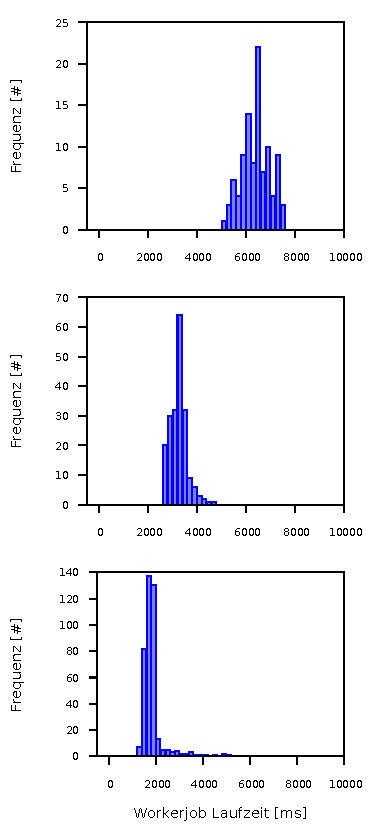
\includegraphics{hist-workerPrimeCpp}
    \caption{Experiment \ref{M1} WorkerJob Laufzeiten aller 25 Iterationen in 50bins.}
    \label{hist-workerPrimeCpp}
  \end{center}
\end{wrapfigure}

%#WorkerJobs
%was amcht ein Workerjob
%IO
%avg(T)
%#messages
%parameter

Dieses Experiment wurde ausgewählt, weil es einen sehr einfachen Fall zeigt, der auch gut skaliert.
Der Algorithmus duchsucht den Bereich $10^{7}$ bis $2 \cdot 10^{7}$ nach Primzahlen und übergibt die Anzahl der gefundenen Primzahlen zusammen mit dem Progress in Echtzeit an den Client.
Die WorkerJobs sind in C++ implementiert, und benötigen keinen Dateisystem IO.
Für Laufzeiten siehe Tabelle \ref{testtable}.

Der Serverteil des \jobScript s teilt den zu durchsuchenden Bereich proportional auf die zur Verfügung stehenden Worker auf.
Somit ist die Anzahl der WorkerJobs immer gleich der Anzahl der Worker.
Stehen mehr Worker zur Verfügung, wird der zu durchsuchende Bereich für jeden Worker kleiner.
Histogramm \ref{hist-workerPrimeCpp} zeigt, dass mittlere WorkerJob Laufzeit annähernd linear mit der Anzahl der verfügbaren Worker sinkt.
Die Gesamtlaufzeit zeigt die erwartete lineare Skalierbarkeit, ersichtlich in Abbildung \ref{runtime-box-workerPrimeCpp} und \ref{runtime-log-workerPrimeCpp}.

Das Messaging Verhalten zwischen Server und Worker benötigt nur einen Roundtrip je Worker Node.
Zu begin sendet der Server eine \CallMessage{} an jede Worker Node, diese senden im 250ms Intervall \UpdateMessage s an den Server, und am Ende möglichst gleichzeitig jeweils eine \ReturnMessage.

Der parallel Workflow skaliert nur dann linear, wenn alle WorkerJobs gleich große Laufzeiten aufweisen.
Bei der Primzahlensuche ist dies im Detail betrachet nicht der Fall, weil großere Zahlen eine größere Laufzeit veruhrsachen und die Zahlen im letzten Block größer sind.


\vspace*{\fill}

\begin{figure}[H]
  \centering
  \begin{minipage}[b]{0.45\textwidth}
    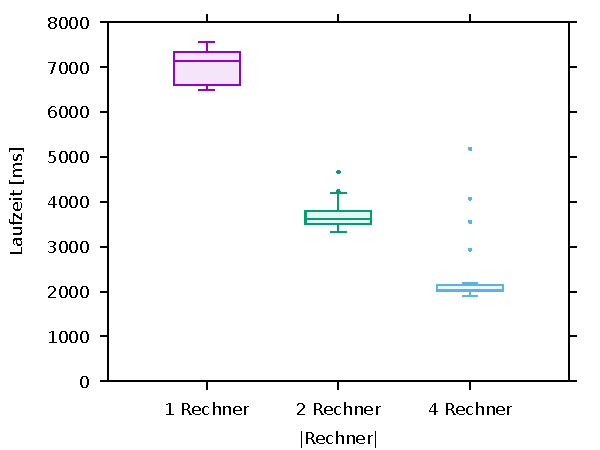
\includegraphics[width=\textwidth]{runtime-box-workerPrimeCpp}
    \caption{Experiment \ref{M1}. Boxplots für Gesamtlaufzeit mit 1, 2, und 4 Worker, und je 25 Iterationen}
    \label{runtime-box-workerPrimeCpp}
  \end{minipage}
  \hfill
  \begin{minipage}[b]{0.45\textwidth}
    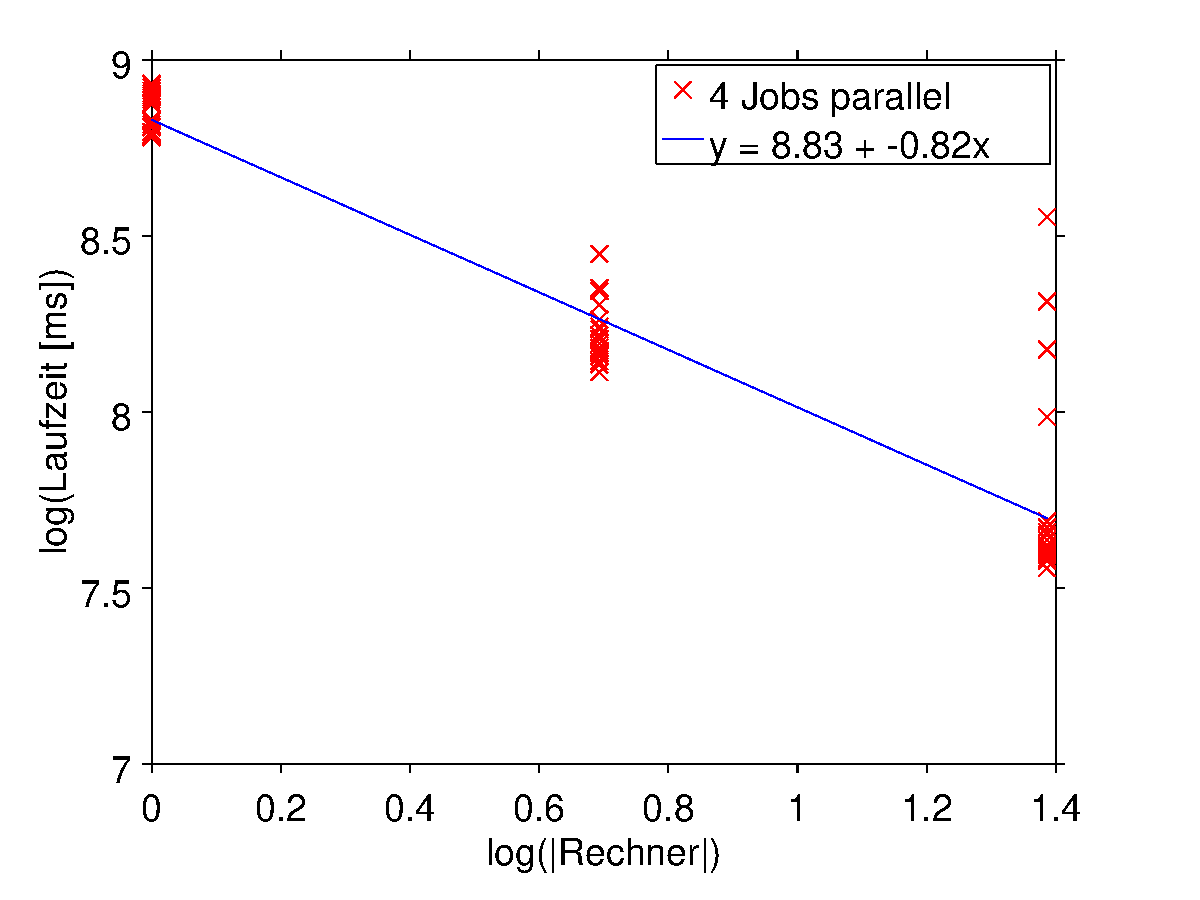
\includegraphics[width=\textwidth]{runtime-log-workerPrimeCpp}
    \caption{Experiment \ref{M1} Gesamtlaufzeiten mit 1, 2, und 4 Workern, und je 25 Iterationen. X und Y Achse logaritmiert.}
    \label{runtime-log-workerPrimeCpp}
  \end{minipage}
\end{figure}
























\clearpage
\subsection{\rgAlgorithmus{} - Pool Workflow}
\label{M2}

\begin{wrapfigure}{r}{0.45\textwidth}
  \vspace{-30pt}
  \begin{center}
    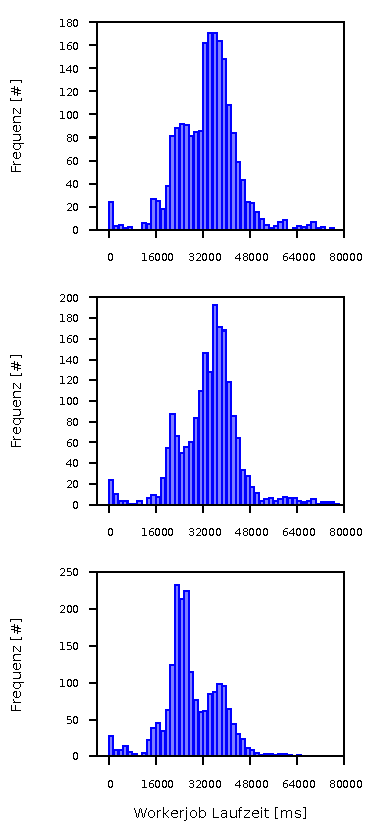
\includegraphics{hist-workerBacc0}
    \caption{Experiment \ref{M2} WorkerJob Laufzeiten aller 25 Iterationen in 50bins. Bei Pool Workflow sollte sich das Histogram nicht ändern.}
    \label{hist-workerBacc0}
  \end{center}
\end{wrapfigure}

Experiment 7.2 zeigt die verteilte Anwendung eines \rgAlgorithmus{}.
Jeder WorkerJob verarbeitet eine von 65 Input-Dateien mit Hilfe eines C++ Programms.
Input- und Output-Dateien werden auf ein AFS Dateisystem geschrieben.
Der Progress wird nur erhöht wenn die Verarbeitung einer Datei abgeschlossen wurde.
Dieses Experiment unterscheidet sich von Experiment \ref{M1} vor allem dadurch, dass deutlich mehr WorkerJobs erzeugt werden als Worker zur Verfügung stehen.
Für Laufzeiten siehe Tabelle \ref{testtable}.

Würde man die Anzahl der parallel laufenden WorkerJobs nicht  nach oben begrenzen, würde es zu Swapping kommen und die Gesamtlaufzeit verschlechtert sich.
Die Begrenzung der Anzahl an parallel laufenden WorkerJobs verhält sich wie Thread Pooling.
Theoretisch sollte dieses Script schlechter skalieren als \ref{M1}, da nach Terminierung eines WorkerJobs ein Roundtrip notwendig ist um den nächsten WorkerJob zu starten.
Insgesamt sind im Vergleich zu Experiment \ref{M1} $n - w$ zusätzliche Roundtrips notwendig, wobei $n$ die Anzahl der WorkerJobs, und $w$ die Anzahl der Worker ist.
Dieser Nachteil macht sich in der Gesamtlaufzeit allerdings kaum bemerkbar, solange ein WorkerJob (wie in diesem Fall) viel länger dauert als ein Roundtrip.

Ein weiterer Grund, warum dieses Experiment schlechter skaliert als Experiment \ref{M1}, ist die ungleiche Verteilung der WorkerJob Laufzeiten.
Wird der WorkerJob mit der längsten Laufzeit als letzter gestartet, wird dieser noch laufen, wenn alle anderen bereits terminiert haben
- oder anders gesagt, es werden nicht alle Ressourcen über die gesamte Laufzeit des Algorithmus genutzt (siehe Abschnitt \ref{schedulerNeeded}).
Sind die Laufzeiten der WorkerJobs im Voraus bekannt, könnte dieses Problem minimiert werden.


\vspace*{\fill}

\begin{figure}[H]
  \centering
  \begin{minipage}[b]{0.45\textwidth}
    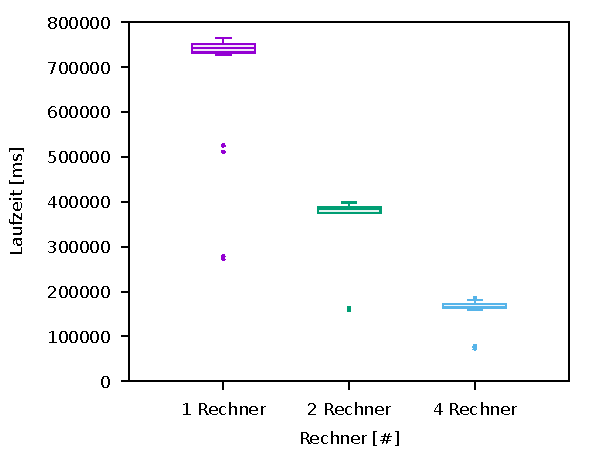
\includegraphics[width=\textwidth]{runtime-box-workerBacc0}
    \caption{Experiment \ref{M2}. Boxplots für Gesamtlaufzeit mit 1, 2, und 4 Worker, und je 25 Iterationen}
    \label{runtime-box-workerBacc0}
  \end{minipage}
  \hfill
  \begin{minipage}[b]{0.45\textwidth}
    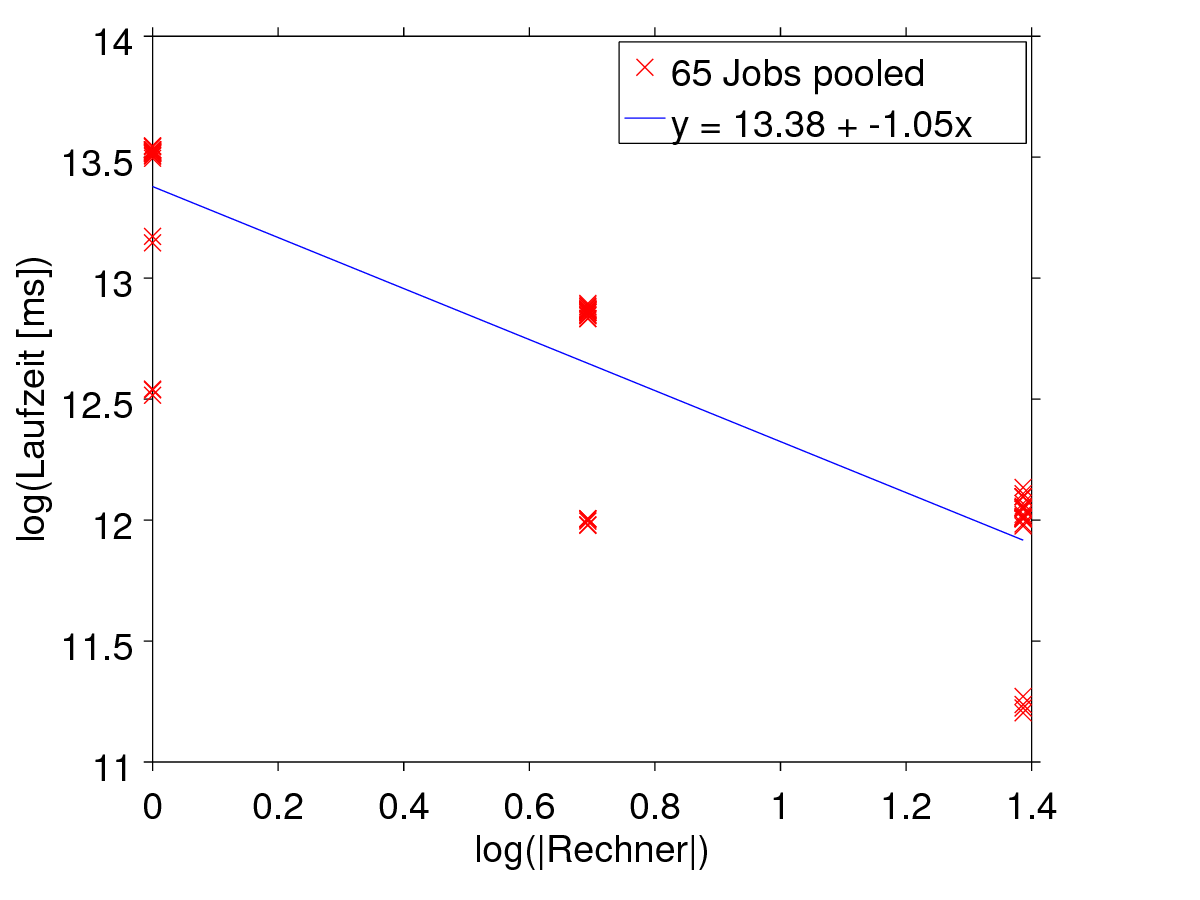
\includegraphics[width=\textwidth]{runtime-log-workerBacc0}
    \caption{Experiment \ref{M2} Gesamtlaufzeiten mit 1, 2, und 4 Workern, und je 25 Iterationen. X und Y Achse logaritmiert.}
    \label{runtime-log-workerBacc0}
  \end{minipage}
\end{figure}



















\clearpage
\subsection{Empty Jobs - Pool Workflow}
\label{M3}

\begin{wrapfigure}{r}{0.45\textwidth}
  \vspace{-30pt}
  \begin{center}
    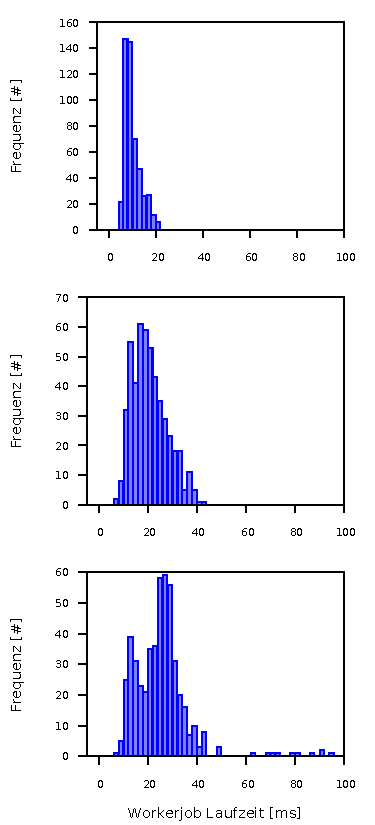
\includegraphics{hist-workerBacc1}
    \caption{Experiment \ref{M3} WorkerJob Laufzeiten aller 25 Iterationen in 50bins.  Bei Pool Workflow sollte sich das Histogram nicht ändern.}
    \label{hist-workerBacc1}
  \end{center}
\end{wrapfigure}

Dieses Experiment soll den durch die Middleware verursachten Overhead bei Verwendung eines Pool Workflows zeigen.
Die im Pool gestarteten WorkerJobs führen keinen Nutz-Algorithmus aus, sie terminieren unmittelbar nach dem Start.
Für Laufzeiten siehe Tabelle \ref{testtable}.
Wie alle anderen Experimente wird auch dieses mit einem, zwei und vier Rechnern mit je vier Workern ausgeführt.

Es zeigt sich, dass der Server bereits mit acht Workern, überlastet ist.
Zu erkennen ist dies am Histogramm in Abbildung \ref{hist-workerBacc1}.
Die Laufzeit von \remoteJob s wird am auftraggebenenden Gerät gemessen, inklusive Roundtrip, Serialisierung, und Workflow Logic.
Das Histogramm zeigt schon bei acht, und vor allem bei 16 Workern viel längere Laufzeiten.
Da die tatsächliche Laufzeit am Worker nahezu null ist und angenommen werden kann, dass die Roundtrip Zeit sich nicht wesentlich veränert hat, muss die zusätzliche Laufzeit dem Server zugeschrieben werden.

Die Message Sequenz ist die selbe wie bei \ref{M2}.
Gleicher Workflow bedeutet immer gleiche Message Sequenz mit Ausnahme der \UpdateMessage s, die hier vernachlässigt werden können.
Die Zeitabstände sind aber geringer, da die WorkerJobs sofort Terminieren.
Erhält der Server von zu vielen Workern Return Messages in kurzen Abständen, wächst die Queue am Server.
Die Auslastung des Servers ist von der Anzahl der Worker, die mit ihm verbunden sind, linear abhängig.
Ein \hcsno{} mit mehreren Worker Ebenen könnte dieses Problem beheben, da es die Serverauslastung logarithmisch von der Gesamtanzahl der Worker abhängig macht.
Ein solches System könnte in einer zukünftgien Arbeit untersucht werden.

\vspace*{\fill}

\begin{figure}[H]
  \centering
  \begin{minipage}[b]{0.45\textwidth}
    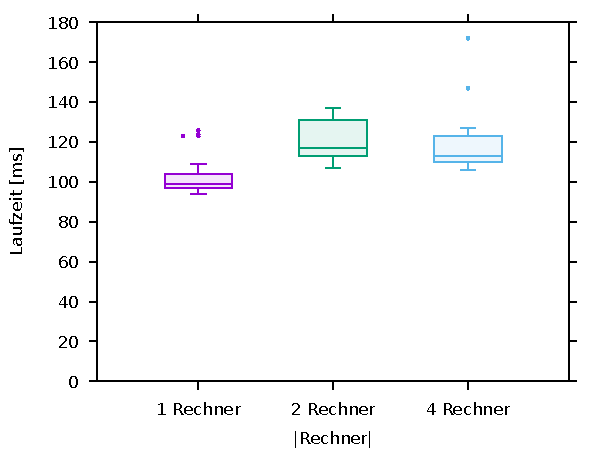
\includegraphics[width=\textwidth]{runtime-box-workerBacc1}
    \caption{Experiment \ref{M3}. Boxplots für Gesamtlaufzeit mit 1, 2, und 4 Worker, und je 25 Iterationen}
    \label{runtime-box-workerBacc1}
  \end{minipage}
  \hfill
  \begin{minipage}[b]{0.45\textwidth}
    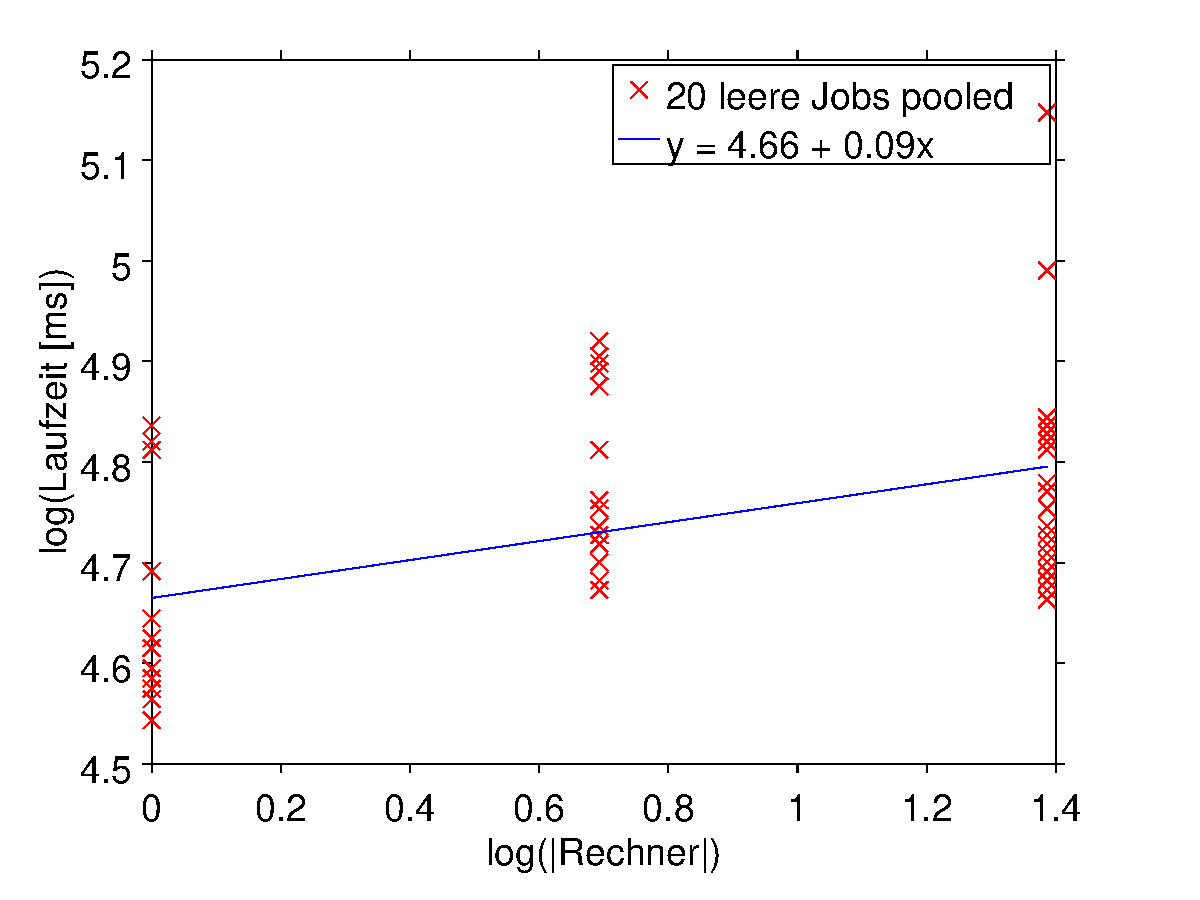
\includegraphics[width=\textwidth]{runtime-log-workerBacc1}
    \caption{Experiment \ref{M3} Gesamtlaufzeiten mit 1, 2, und 4 Workern, und je 25 Iterationen. X und Y Achse logaritmiert.}
    \label{runtime-log-workerBacc1}
  \end{minipage}
\end{figure}





















\clearpage
\section{Webclient Tests}
\subsection{\scheduler{} Fail}
\label{schedulerNeeded}
Folgendes Script führt 12 WorkerJobs mit zufälliger Laufzeit zwischen einer und 15 Sekunden in einem Pool von drei Workern aus.

Die Summe der Worker Laufzeiten beträgt 49s, durch die Anzahl der Worker geteilt sollte die Gesamtlaufzeit 17s nicht überschreiten.
Die Laufzeit beträgt aber 21s (siehe Tabelle \ref{testtable}), das System war also zu weniger als 84\% ausgelastet.
Abbildung \ref{fig:gant0} zeigt die nicht genutzten Worker Ressourcen im Gant Chart.
Ungünsige Konstellationen können eine noch weitaus schlechtere Auslastung zur Folge haben.
Bei unregelmäßigen WorkerJob Laufzeiten können andere \scheduler -Implementierungen für eine bessere Auslastung sorgen.
Das \scheduler{} Interface hat derzeit die Einschränkung, dass die Worker Nodes beim Start des Workflows bekannt sein müssen.

\begin{figure}[H]
  \begin{center}
    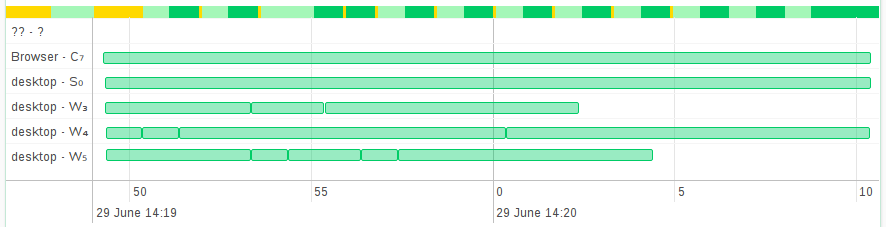
\includegraphics[width=1\textwidth]{gant}
    \caption{Gant Chart von 12 Workerjobs mit zufälliger Laufzeit.
    \label{fig:gant0}
    $W_4$ verzögert den Abschluss von $S_0$ und $C_7$ und verursacht dadurch eine und schlechte Systemauslastung. Diese Abbildung ist ein Screenshot des Webclients.}
  \end{center}
\end{figure}
\noindent



\subsection{Client Überlastung}
\label{overload}
Folgendes Script führt 20 ‘leere’ WorkerJobs in einem Pool von drei Workers aus.
Es ist das selbe Script das in Experiment \ref{M3} verwendet wurde.
Experiment \ref{M3} hat gezeigt, dass der CLI-Client leere Jobs mit bis zu 4 Worker Nodes verarbeiten kann.
Dieses Experiment wird mit 3 Worker Nodes ausgeführt, um eine Überlastung des Servers auszuschließen.

Am Webclient benötigt es 1064ms, der CLI-Client nur 103ms.
Der Webclient muss überlastet sein, da der Rest des Systems sich nicht geändert hat.
Auf den ersten Blick lässt Abbildung \ref{fig:gant2} vermuten, dass der Server überlastet ist.
Berücksichtigt man aber das $S_0$ am Client erstellt wurde, und Laufzeiten immer auf dem erstellenden Device gemessen werden, kann diese Fehlinterpretation erklärt werden.
Der Webclient ist, auch wenn die Anzahl der Worker korrekt dimensioniert wurde, anfällig für Überlastungen da \GUI{} Aktualisierungen rechenintensiv sind.


%Kurz nachdem der letzte WorkerJob auf $W_4$ terminiert, terminiert der ServerJob $S_0$ und danach der \RootJob{} am $C_7$.
%Die Verzögerung, bestehend aus Netzwerklatenz und Verarbeitungszeit der return Transition, ist minimal - in dieser Darstellung kaum sichtbar im Vergleich zu \ref{overload}.
%'Leer' bedeutet sie terminieren direkt nach dem Start. TODO |msg|=const -> runtime gering -> overhead macht maximialen teil aus.
%Abbildung \ref{fig:gant2} zeigt eine Überlastung des Clients oder Servers, erkennbar an der großen Zeitspanne zwischen dem Ende des letzten WorkerJobs und dem Ende des ServerJobs.
%Diese Verzögerung setzt sich zusammen aus Netzwerklatenz und onReturn Transition Verarbeitung, jeweils für den Server und Client - auf Server und Client, weil der auf $S_0$ ausgeführte Job auf $C_7$ erstellt wurde und die Joblaufzeit am auftraggebenden Gerät gemessen wird.
%Ob die Verzögerung auf dem Server oder Client entstanden ist, kann anhand dieses Diagramms nicht bestimmt werden.
%Eine Erweiterung der Visualisierung, die die Queueläge zeigt, würde die Identifizierung des überlasteten Geräts ermöglichen.
\begin{figure}[H]
  \begin{center}
    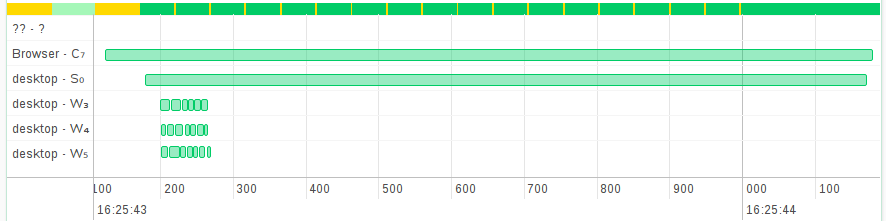
\includegraphics[width=1\textwidth]{gant2}
    \caption{Gant Chart von 20 Workerjobs mit minimaler Laufzeit.
    \label{fig:gant2}
    Das Scheduling der WorkerJobs ist akzeptabel. $C_7$ terminiert spät aufgrund einer Überlastung des Webclients. Diese Abbildung ist ein Screenshot des Webclients.}
  \end{center}
\end{figure}
\noindent
